
\documentclass[manuscript,screen,review, nonacm]{acmart}

\usepackage{graphicx}
\usepackage{float}
\usepackage{caption}
\usepackage{subcaption}


%%
%% end of the preamble, start of the body of the document source.
\begin{document}

%%
%% The "title" command has an optional parameter,
%% allowing the author to define a "short title" to be used in page headers.
\title{Explanation and Analysis of Models Chosen}

%%
%% The "author" command and its associated commands are used to define
%% the authors and their affiliations.
%% Of note is the shared affiliation of the first two authors, and the
%% "authornote" and "authornotemark" commands
%% used to denote shared contribution to the research.
\author{Harvey Kwong}
\email{harveykw@buffalo.edu}
\author{Jacob DeRosa}
\email{jderosa3@buffalo.edu}
\affiliation{%
  \institution{University at Buffalo}
  \city{Buffalo}
  \state{New York}
  \country{USA}
}


\maketitle

\section{Introduction}

Following thorough data cleaning and exploratory data analysis, we identified 15 key predictor features. Our objective is to utilize these predictors to classify whether a given sample of *Neisseria gonorrhoeae* exhibits super resistance to specific antibiotics. In this study, resistance to azithromycin serves as the target label for our classification models. Since the target variable is binary (either true or false), we implemented and evaluated six different types of classifiers:
  
  \begin{itemize}
      \item \href{https://scikit-learn.org/stable/modules/generated/sklearn.neighbors.KNeighborsClassifier.html}{K-Nearest Neighbors}
      \item \href{https://scikit-learn.org/stable/modules/naive_bayes.html}{Naive Bayes}
      \item \href{https://scikit-learn.org/stable/modules/generated/sklearn.linear_model.LogisticRegression.html}{Logistic Regression}
      \item \href{https://scikit-learn.org/stable/modules/svm.html}{Support Vector Machine (SVM)}
      \item \href{https://www.tensorflow.org/api_docs/python/tf/keras/Sequential}{Neural Network} - (Not from Class) Harvey Kwong's custom architecture
      \item \href{https://xgboost.readthedocs.io/en/stable/get_started.html}{Extreme Gradient Boosting (XGBoost)} - (Not from class)
  \end{itemize}
  


  \section*{K - Nearest Neighbors}


    We selected K-Nearest Neighbors as one of the models for our analysis. 
    KNN is a good fit for our problem due to the relatively low dimensionality 
    of the dataset, where we focused on only the most significant features identified 
    during our exploratory data analysis process. By reducing the number of features, KNN's performance 
    improves, as it works best when our data is not at a very high dimension.

    For this model, we chose to use 5 neighbors, as this configuration 
    provided the most balanced results. Fewer neighbors made the model more 
    sensitive to noise and overfitting, while more neighbors reduced its ability 
    to capture important variations. Overall, KNN performed strongly, achieving 
    approximately 96\% accuracy in predicting azithromycin resistance. The extended 
    metrics for this model are as follows:


  \begin{table}[H]
    \centering
    \begin{tabular}{@{}lc@{}}
        \toprule
        \textbf{Metric} & \textbf{Score} \\ \midrule
        Accuracy  & 0.9647 \\
        Precision & 0.9714 \\
        Recall    & 0.9647 \\
        F1 Score  & 0.9667 \\ \bottomrule
    \end{tabular}
    \caption{Performance Metrics for K-Nearest Neighbors}

\end{table}
  
  \begin{figure}[H]
      \centering
      \begin{subfigure}{0.45\textwidth}
          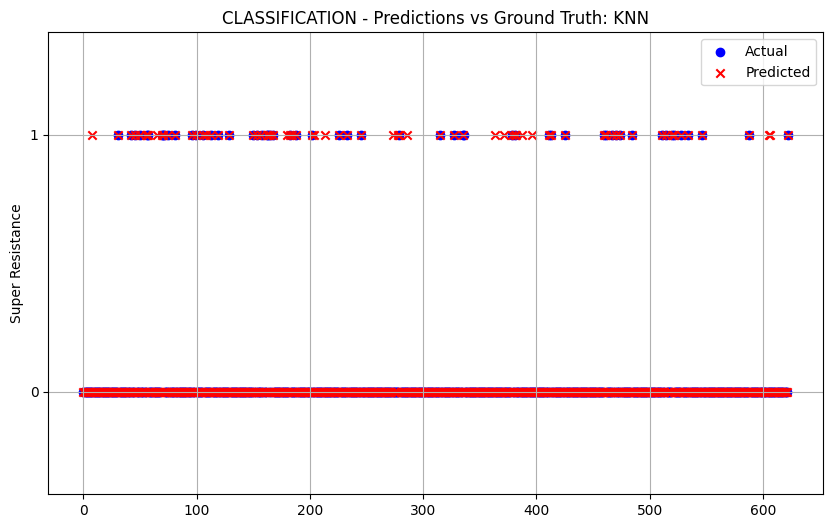
\includegraphics[width=\linewidth]{figs/KNN1.png}
          \caption{K-Nearest Neighbors Predictions vs Ground Truth}

      \end{subfigure}
      \hfill
      \begin{subfigure}{0.45\textwidth}
          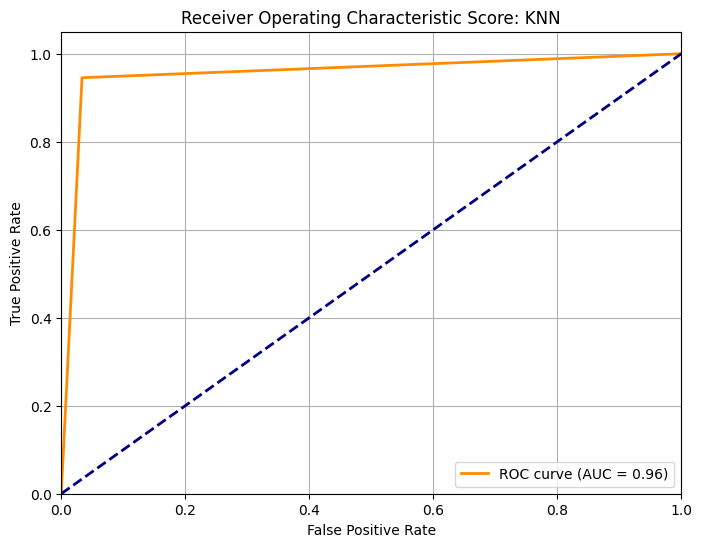
\includegraphics[width=\linewidth]{figs/knn2.png}
          \caption{K-Nearest Neighbors ROC curve}

      \end{subfigure}
      \caption{K-Nearest Neighbors}

  \end{figure}

  \section*{Naive Bayes}


    We chose to implement Naive Bayes as one of our classification models. 
    Naive Bayes is well-suited to our problem due to its efficiency and simplicity, 
    especially when dealing with binary classification tasks like predicting antibiotic 
    resistance. The model assumes that the features are independent, which, while a 
    simplification because many things are interconnected in biology -- performed surprisingly 
    well in our modelling.  Given the relatively reduced number of features in our dataset, 
    Naive Bayes was an appropriate choice as it tends to work well even with limited data.

    Additionally, Naive Bayes requires minimal computational resources, 
    which makes it advantageous for fast predictions. Although it does not capture 
    feature interactions, it still correctly predicted azithromycin resistance approximately 91\% of the time. 
    Our extended metrics for this model are as follows:

  \begin{table}[H]
    \centering
    \begin{tabular}{@{}lc@{}}
        \toprule
        \textbf{Metric} & \textbf{Score} \\ \midrule
        Accuracy  & 0.9197 \\
        Precision & 0.9545 \\
        Recall    & 0.9197 \\
        F1 Score  & 0.9298 \\ \bottomrule
    \end{tabular}
    \caption{Performance Metrics for Naive Bayes}

\end{table}
  
  \begin{figure}[H]
      \centering
      \begin{subfigure}{0.45\textwidth}
          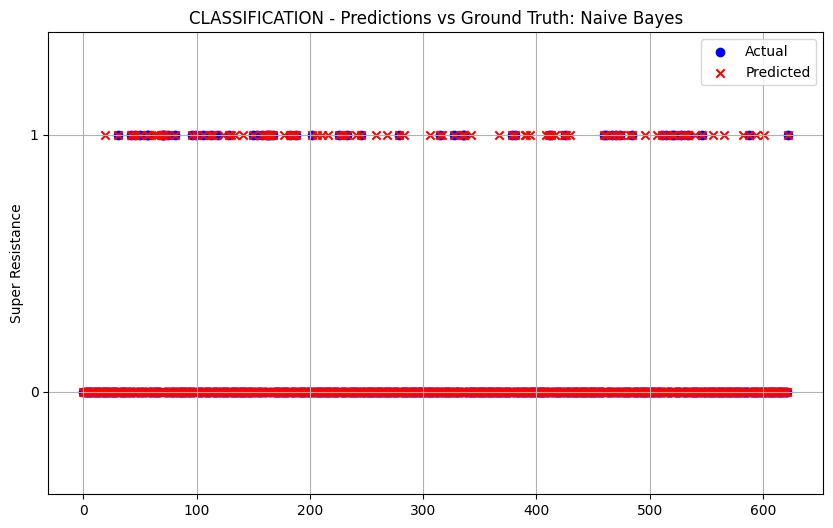
\includegraphics[width=\linewidth]{figs/bayes1.png}
          \caption{Naive Bayes Predictions vs Ground Truth}

      \end{subfigure}
      \hfill
      \begin{subfigure}{0.45\textwidth}
          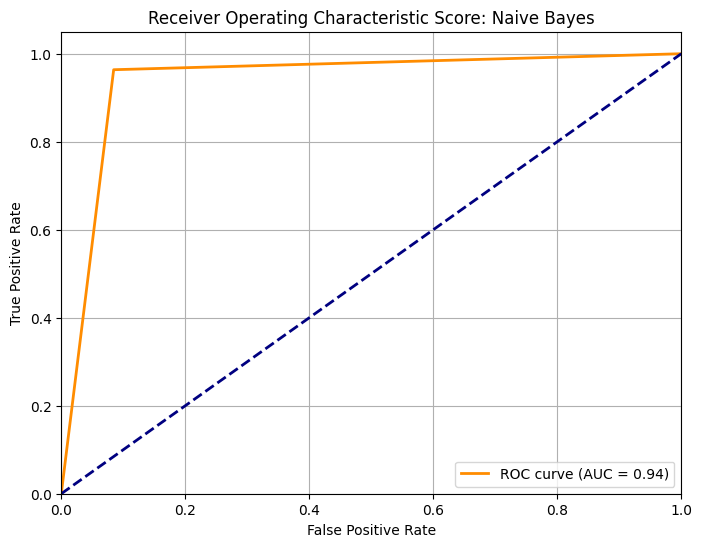
\includegraphics[width=\linewidth]{figs/bayes2.png}
          \caption{Naive Bayes ROC curve}

      \end{subfigure}
      \caption{Naive Bayes}

  \end{figure}



  \section*{Logistic Regression}


  We chose to include Logistic Regression as one of the models for our classification task. 
  Logistic Regression is a commonly used algorithm for binary classification problems like 
  ours, where the goal is to predict azithromycin resistance. One of the main advantages of 
  Logistic Regression is its simplicity and interpretability, as it provides clear 
  probabilistic outputs. This makes it particularly useful for understanding the 
  relationship between the predictor variables and the target label. Though in our model,
  we thresholded the predicted values. Values above 0.5 went to positive, and those below went
  to negative.

  Since our dataset contains well-processed and balanced features, 
  Logistic Regression was able to achieve a solid performance without much additional 
  complex tuning. Despite using a max iteration limit of 10, the model demonstrated reliable 
  results, with an accuracy of around 95\%. Our extended metrics for this model are as follows:

  \begin{table}[H]
    \centering
    \begin{tabular}{@{}lc@{}}
        \toprule
        \textbf{Metric} & \textbf{Score} \\ \midrule
        Accuracy  & 0.9502 \\
        Precision & 0.9681 \\
        Recall    & 0.9502 \\
        F1 Score  & 0.9550 \\ \bottomrule
    \end{tabular}
    \caption{Performance Metrics for Logistic Regression}

\end{table}
  
  \begin{figure}[H]
      \centering
      \begin{subfigure}{0.45\textwidth}
          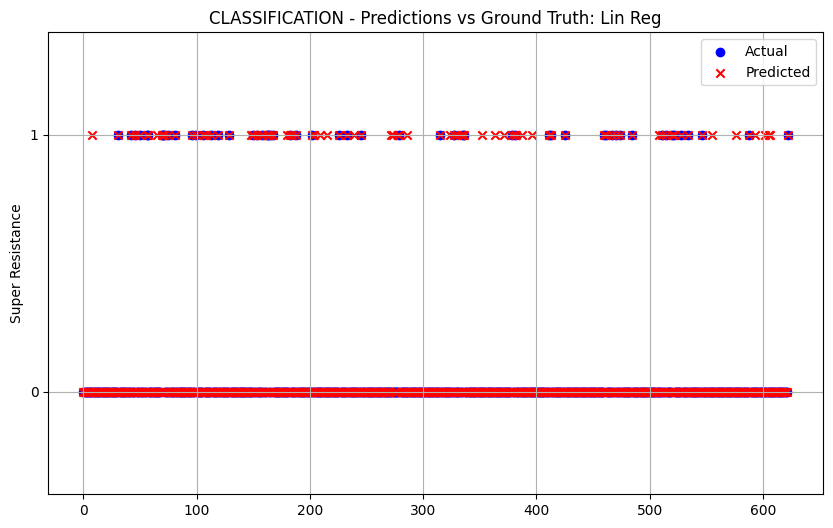
\includegraphics[width=\linewidth]{figs/lin1.png}
          \caption{Logistic Regression Predictions vs Ground Truth}

      \end{subfigure}
      \hfill
      \begin{subfigure}{0.45\textwidth}
          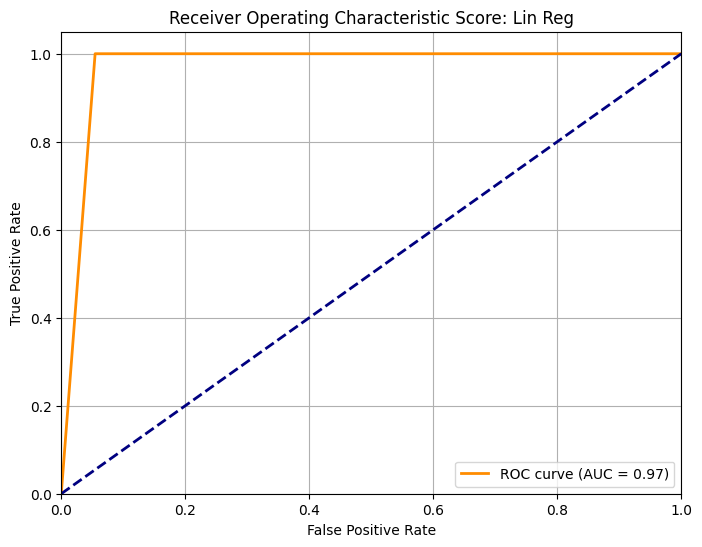
\includegraphics[width=\linewidth]{figs/lin2.png}
          \caption{Logistic Regression ROC curve}

      \end{subfigure}
      \caption{Logistic Regression}

  \end{figure}


  \section*{Support Vector Machine (SVM)}

  We chose to include support vector machines as one of the models for our 
  classification task. SVM is a powerful algorithm for binary classification problems. 
  It works by finding an optimal hyperplane that separates the classes with the largest 
  margin, making it effective in cases where the data is not linearly separable. SVM is 
  well-suited to this problem as it can handle non-linear decision boundaries using 
  various kernels. For our implementation, we used the default polynomial kernel and set the maximum number of iterations to 
  10 to ensure computational efficiency while maintaining acceptable performance. 
  Despite the iteration limit, SVM performed reasonably ok, achieving an accuracy 
  of approximately 87\%. Our extended metrics for our SVM model are as follows:

\begin{table}[H]
    \centering
    \begin{tabular}{@{}lc@{}}
        \toprule
        \textbf{Metric} & \textbf{Score} \\ \midrule
        Accuracy  & 0.8732 \\
        Precision & 0.9249 \\
        Recall    & 0.8732 \\
        F1 Score  & 0.8911 \\ \bottomrule
    \end{tabular}
    \caption{Performance Metrics for Support Vector Machine}
\end{table}

\begin{figure}[H]
    \centering
    \begin{subfigure}{0.45\textwidth}
        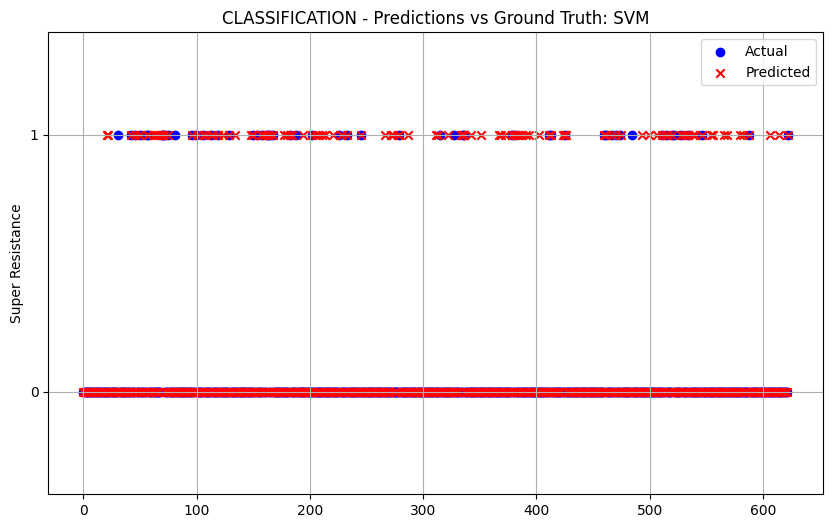
\includegraphics[width=\linewidth]{figs/svm1.png}
        \caption{SVM Predictions vs Ground Truth}
    \end{subfigure}
    \hfill
    \begin{subfigure}{0.45\textwidth}
        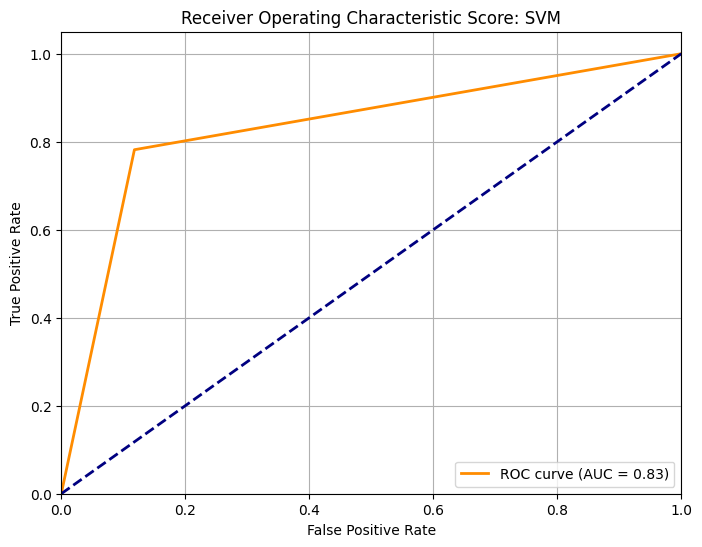
\includegraphics[width=\linewidth]{figs/svm2.png}
        \caption{SVM ROC Curve}
    \end{subfigure}
    \caption{Support Vector Machine}
\end{figure}

\section*{Neural Network}

We included a custom Neural Network as one of the models for our classification task. 
Neural networks are highly flexible and capable of capturing complex patterns in data, 
making them suitable for problems where non-linear relationships between features and the 
target label exist. Given the relatively simple structure of our dataset, we designed a 
straightforward architecture to avoid overfitting and any other unnecessary complexities.

Our custom architecture consists of two hidden layers with 8 and 4 neurons, respectively, 
both using the RELU activation function. For the output layer, we used a single neuron with 
a sigmoid activation function, which is the norm for binary classification tasks. We compiled 
the model with the Adam optimizer and binary cross-entropy loss, ensuring efficient training 
with a learning rate of 0.1. Adam will automatically adjust the learning rate as it sees fit.

Despite the simplicity of the architecture, the neural network performed fine, achieving 
an accuracy of approximately 90\%. We trained the model for 10 epochs, to enable easier 
comparisons with our other models which have had their maximum iterations set to 10. Our neural
network did not perform as well as logistic regression despite having a more complicated
structure and presumably higher computational cost. It is likely better to use logistic regression
on our dataset compared to our neural network with our current choice of hyperparameters.
i expect that if we were to increase the number of hidden units and epochs, we would see much better
performance, though at a higher cost. Our extended metrics for this neural 
network model are as follows:

\begin{table}[H]
    \centering
    \begin{tabular}{@{}lc@{}}
        \toprule
        \textbf{Metric} & \textbf{Score} \\ \midrule
        Accuracy  & 0.9053 \\
        Precision & 0.9543 \\
        Recall    & 0.9053 \\
        F1 Score  & 0.9192 \\ \bottomrule
    \end{tabular}
    \caption{Performance Metrics for Neural Network}
\end{table}

\begin{figure}[H]
    \centering
    \begin{subfigure}{0.45\textwidth}
        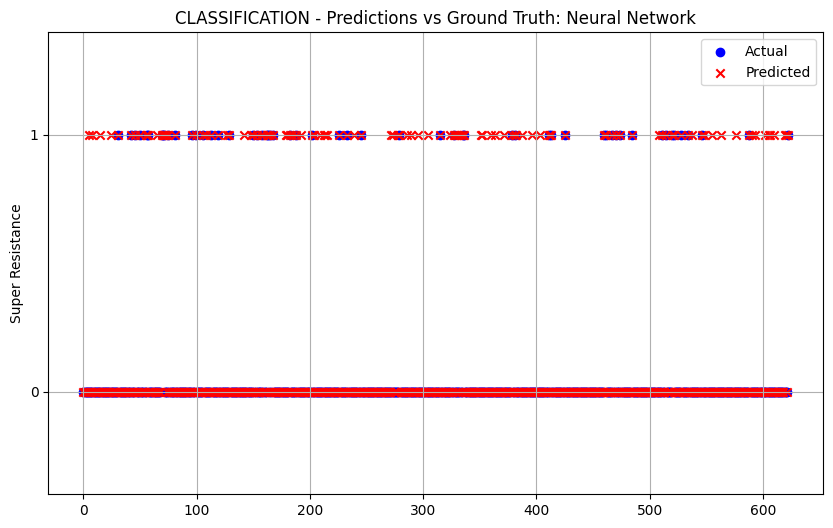
\includegraphics[width=\linewidth]{figs/nn1.png}
        \caption{Neural Network Predictions vs Ground Truth}
    \end{subfigure}
    \hfill
    \begin{subfigure}{0.45\textwidth}
        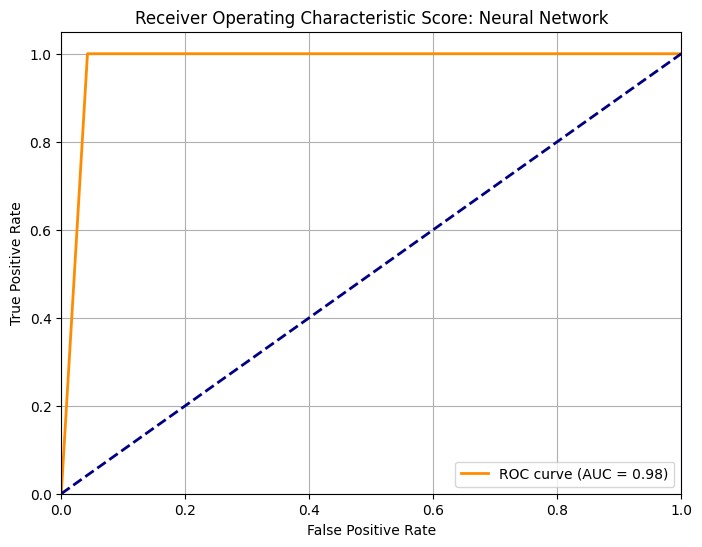
\includegraphics[width=\linewidth]{figs/nn2.png}
        \caption{Neural Network ROC Curve}
    \end{subfigure}
    \caption{Neural Network}
\end{figure}



\end{document}